%%
%% precntnt.tex - LaTeX2e thesis class
%%
%% Copyright (C) 2012 Mathew Topper <damm_horse@yahoo.co.uk>
%%
%% This file is part of the University of Edinburgh, Department of
%% Engineering LaTeX2e thesis template.
%% 
%% The University of Edinburgh, Department of Engineering LaTeX2e thesis
%% template is free software: you can redistribute it and/or modify
%% it under the terms of the GNU General Public License as published by
%% the Free Software Foundation, either version 3 of the License, or
%% (at your option) any later version.
%% 
%% The University of Edinburgh, Department of Engineering LaTeX2e thesis
%% template is distributed in the hope that it will be useful,
%% but WITHOUT ANY WARRANTY; without even the implied warranty of
%% MERCHANTABILITY or FITNESS FOR A PARTICULAR PURPOSE.  See the
%% GNU General Public License for more details.
%% 
%% You should have received a copy of the GNU General Public License
%% along with the University of Edinburgh, Department of Engineering
%% LaTeX2e thesis template.  If not, see <http://www.gnu.org/licenses/>.
%%
%%
%%   ABOUT
%%
%% This is frontmatter prior to the contents for a Latex2e template which
%% corresponds to the regulations regarding layout of a thesis submitted
%% within the University of Edinburgh School of Engineering. It is not
%% `official', but conforms as best as possible to the regulation as detailed
%% at:
%%
%% http://www.ed.ac.uk/schools-departments/science-engineering/current-students/
%% research/submitting-thesis
%%
%% Please feel free to alter the template to your own liking, but note that
%% the template is made available under the GNU GPL and must be similarly
%% licenced should you wish to release your modified template.
%%
%%
%%   CREDITS
%%
%% This template is an amalgamtion of an existing Edinburgh University,
%% Electrical Engineering PhD Thesis class file (jthesis-v1.cls) authored by
%% George S Taylor which was released under the GNU GPL.
%% Code is included from the dmathesis class Written by M. Imran
%% for a thesis according to the university of Durham regulation, which was
%% released without copyright. It also contains ideas (possibly code) from the
%% Princeton thesis class file (PrincetonThesis.cls), authored by Mike Nolta.
%% Mathew Topper, Eoghan Maguire and Bill Edwards forsaw the need to maintain a
%% more recent latex implementation of the thesis regulations and thus, this
%% project was born. It is hoped that the template will be maintained by the
%% Edinburgh Engineering PhD community once released.
%%
%%
%%   RECORD OF REVISIONS
%%
%%     Date      Programmer        Description of change
%%     ====      ==========        =====================
%%   21/06/10    Mathew Topper     Original Code
%%   19/10/10                      Renamed to precntnt.tex
%%                                 frontmtr.tex now does all
%%                                 front matter add can be
%%                                 used in an include statement
%%
%%

%% INPUT THIS FILE USING THE /makefrontmatter{} COMMAND OR THE FORMATTING
%% WON'T WORK PROPERLY

\phantomsection%
\addcontentsline{toc}{chapter}{Mission Statement}%
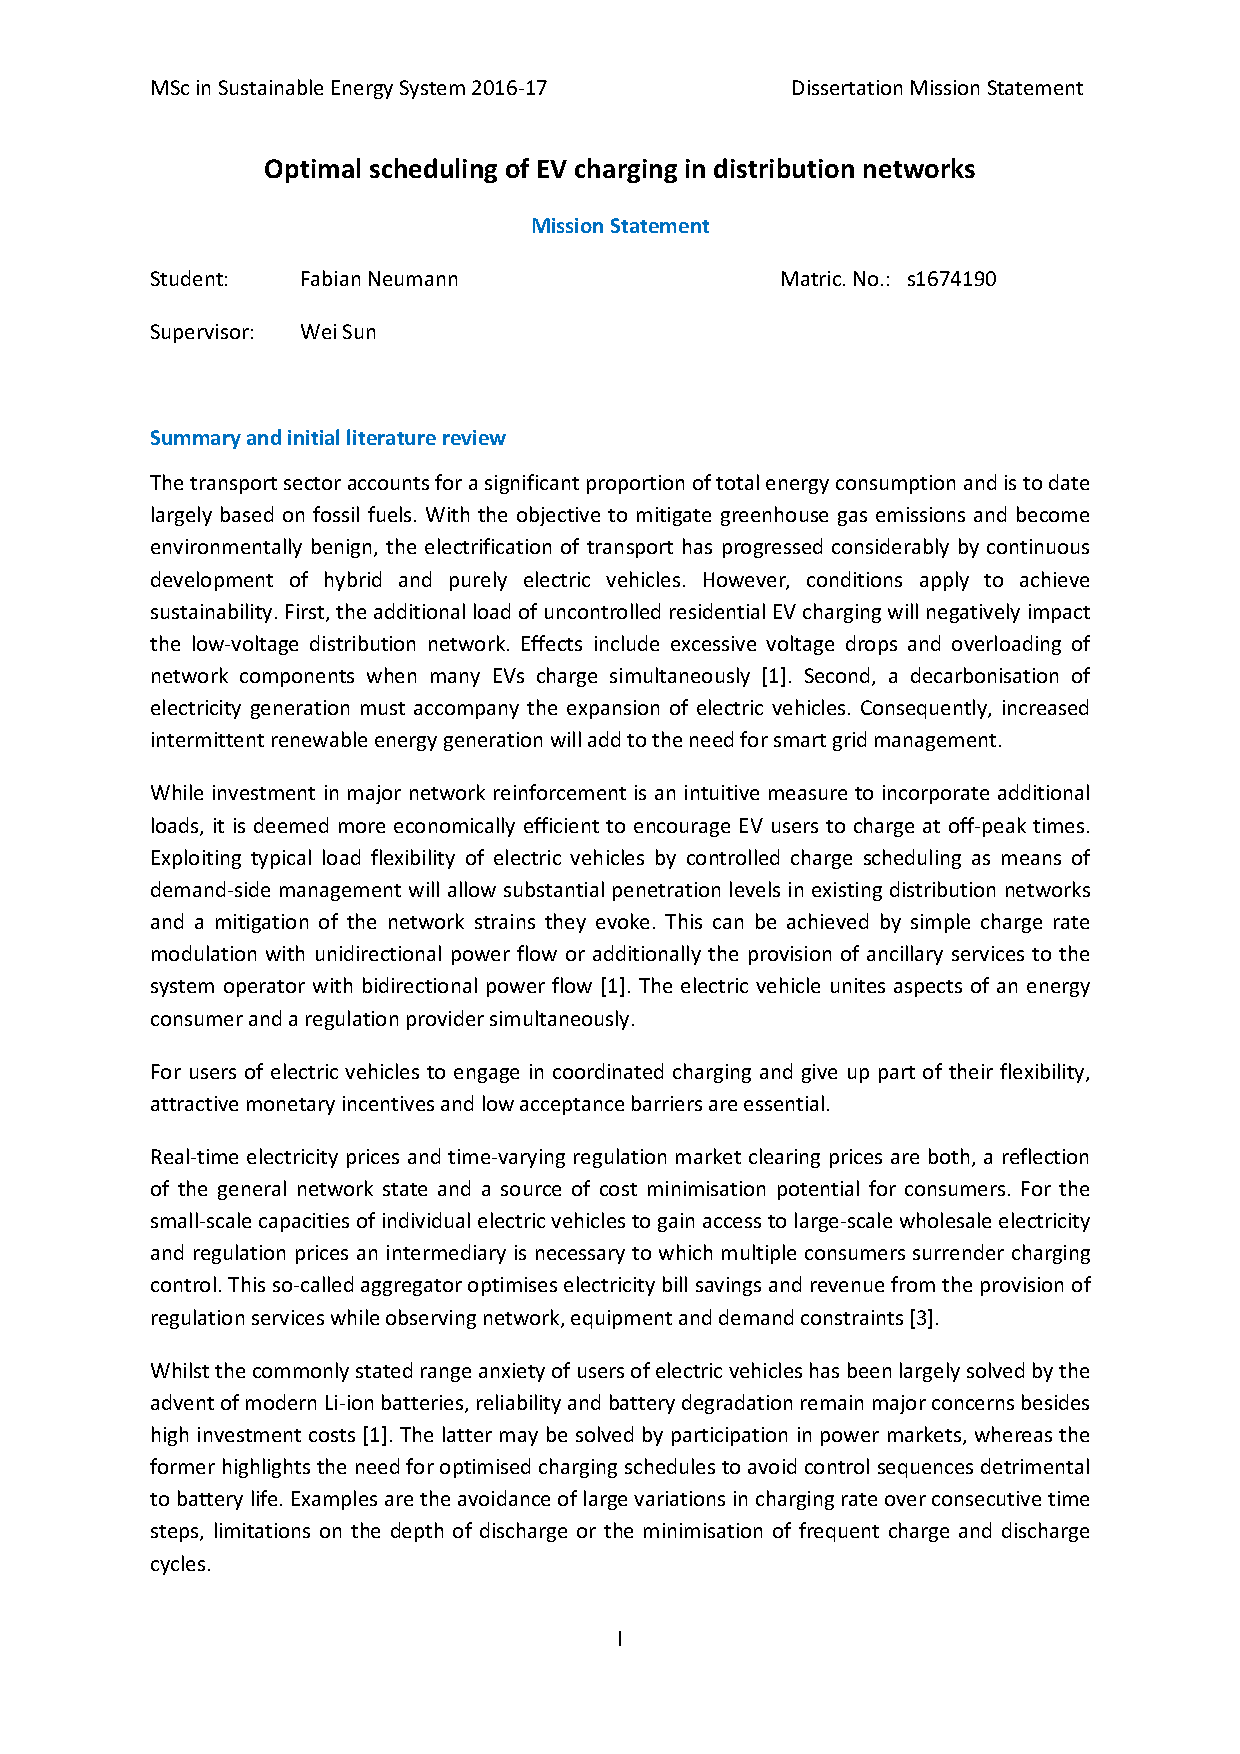
\includepdf[pages={1-6},scale=1.0]{figures/MissionStatement_NeumannF}
\mbox{}
\thispagestyle{empty}
\newpage
\cleardoublepage

%%%% ABSTRACT
\abstract{
	
The transport sector accounts for a significant proportion of total energy consumption and is to date largely based on fossil fuels. Mitigation of greenhouse gas emissions via the large-scale electrification of road transport will likely deteriorate voltage profiles and overload network equipment in distribution networks. Controlling the charging schedule of electric vehicles in a centralised and coordinated manner provides a potential solution to mitigate the issues and could defer the investment on upgrading the network infrastructures.

In this work, a robust cost-minimising unidirectional day-ahead scheduling routine for charging electric vehicles overnight in residential low voltage distribution networks is presented that observes local network, equipment and charging demand constraints in a stochastic environment. To reduce the computational complexity, a linear power flow approximation is utilised. The modelled environment involves uncertain residential electricity demand, market prices, and the mobility behaviour of electric vehicle owners including stochastic daily trip distances, arrival and departure times. Knowledge about the probability distributions of these parameters is used to hedge risks regarding the cost of charging, network overloadings, voltage violation and charging reliability.

The results provide an insight into the impact of uncertainty and the effectiveness of addressing particular aspects of risk during optimisation. Particularly, consideration of temporally variable household-level demand peaks and planning with more conservative estimates of initial battery charge levels increased the reliability and technical feasibility of optimised schedules. It is further outlined that the introduction of dynamic grid levies, which amplify the effect of variable electricity prices, constitutes a key determinant of cost saving potential by demand side management that could incur only minor fiscal implications.

}

%%%% DECLARATION

%% Use a custom declaration

% \declaration{I did it.}

%% Use the standard regulation declaration. Enter your
%% name for the signature line.

\standarddeclaration{Fabian Neumann, 15 August 2017, Edinburgh}

%%%% ACKNOWLEDGEMENTS

%\acknowledgements{%
%I'd like to thank Danger Mouse, for being so awesome.}

